\documentclass[../book.tex]{subfiles}
\graphicspath{{\subfix{../images/}}}

\begin{document}
\chapter{Essentials for Physics}
\begin{introduction}[Contents]
\item Vectors
\item Modeling Real-World Scenarios
\item Properties of Graphs
\item Using a Graphing Calculator
\end{introduction}
\noindent This chapter will begin to look into how Algebra 2 can manifest itself in real life situations. And the easiest way to see that is through the study of physics! Now what is physics you may ask? Well since this isn't physics class, I’ll give you a mathematical definition. \textit{Physics attempts to condense our world into a model upon which we can predict things with mathematics}. For example, when you say “whatever comes up, must come down”, that involves math. Now we’re not going to delve too much into this but we'll graze some things that would be nice to know. So without further ado, let’s jump into the world of actual applications (now you can’t say Algebra 2 has no point).
\section{Vectors}
\noindent We begin our discussion of physics by discussing vectors.

Now you may be asking what is a vector? Now depending on how many math classes you have taken, or how many you will take, there are varying levels of complexity to this definition. Since you are an incoming freshman, let’s give you a simple one that will work for our purposes: \textit{A vector represents number or quantity in a specific direction}. 

\begin{wrapfigure}{r}{5cm}
    \begin{tikzpicture}[xscale=0.4,yscale=0.4]
        \draw[<->] (-1,0) -- (10,0) node[right] {$x$};
        \draw[<->] (0,-1) -- (0,10) node[above] {$f(x)$};
        \draw[->,blue,thick] (2,3) -- (7.86,6.86) node[midway,sloped,above=1mm] {vector};
        \draw[dashdotted,red] (2,3) -- (8,3) node[midway,below=1mm] {$6$};
        \draw[dashdotted,red] (8,3) -- (8,7) node[midway,right=1mm] {$4$};
        \filldraw (2,3) circle[radius=5pt] node[anchor=north east] {$A$};
        \filldraw (8,7) circle[radius=5pt] node[anchor=south west] {$B$};
    \end{tikzpicture}
\end{wrapfigure}

Usually when we discuss vectors, we bring in the discussion of scalars. Scalars are just numbers. For example, the number $12$, is a scalar. $-12$ is a scalar. Any number that just persists and doesn't have any direction to account for is a scalar. So an easier way to define vector is just a scalar with a direction.

So what does a vector look like? A vector is essentially a point with an arrow being drawn from a second point to it. An image is shown to the right.

With the notion of the vector, we get into the concept of the tail and the head. Usually vectors are drawn from tail to head, so you start at some point, and draw to the end point. Now what would this look like mathematically? 

A vector can be represented three different ways: $$\vec{v}=a\hat{i}+b\hat{j} \hspace{15mm} \vec{v}=<a,b> \hspace{15mm} \vec{v}=\binom{a}{b}.$$
For simplicity, we will stick to the first two (primarily the second) to avoid confusion.

Now you may have noticed the $\hat{i}$ (pronounced $i$-hat) and $\hat{j}$ (pronounced $j$-hat) next to the variables $a$ and $b$ respectively. What do those mean? Well those represent unit vectors. Unit vectors are basically a fancy word for saying a vector has a length of $1$ and has some direction. Now these are next to the variables $a$ and $b$ because they tell us how far to go in each direction.  $\hat{i}$ represents the $+x$-direction, so we go $a$ units in the $+x$ direction. $\hat{j}$ represents the $+y$-direction, so we go $b$ units in the $+y$ direction. And as a result, we obtain the vector, $<a,b>$.

When we discuss the difference between scalars and vectors, this question will be answered: what are some physical concepts that might be vectors or scalars? Well since we’re in physics let’s start with two easy concepts $-$ \textit{distance} versus \textit{displacement}. Below, we list the definitions of each: \begin{itemize}
    \item \textit{Distance} measures the total steps traveled from the starting point to the end point.
    \item \textit{Displacement} measures your position \textbf{relative} to the starting point.
\end{itemize}
To emphasize the difference between the two, let’s suppose we had a $1-D$ system (a line). Let’s say Quinn wants to walk across the line for his daily dose of exercise. Suppose he walks $5$ metres in the $+x$ direction and $10$ metres in the $-x$ direction. What is the distance Quinn traveled? Also what is Quinn’s displacement?

To calculate the distance Quinn traveled, we say he went $5$ metres, so he’s at $5$, then he traveled an additional $10$ metres, so his total distance traveled is $15$ metres.  To calculate Quinn’s displacement, we say he went $5$ metres in the positive $x$-direction, then he traveled back $10$ metres in the negative $x$-direction. So, his displacement is $5-10=-5$ meter.

Notice the difference between he two? Distance doesn't care for direction; it just cares that you traveled. Displacement however cares about how you travel. So going back and forth can affect the sign of our displacement.  This means that displacement is a vector and distance is a scalar.
\subsection{Vector and Scalar Properties}
\noindent This section is going to be very definition-heavy.

Vectors exhibit interesting behavior when we do operations with them.  Let's begin with adding vectors.  

Consider vectors $\vec{v_1}=<a,b>$ and $\vec{v_2}=<c,d>$.  Similar to complex numbers, you should assume that we add each component.  This means that $\vec{v_1}+\vec{v_2}=<a+c,b+d>$.  It's important to also understand how this is graphed since vectors are a very visual subject.  Below are images of how they are graphed.

\begin{figure}[!h]
    \centering
    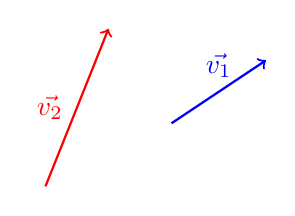
\begin{tikzpicture}[xscale=0.4,yscale=0.4]
        \draw[->,red,thick] (-3,-3) -- (-1,2) node[midway,left=0.5mm] {$\vec{v_2}$};
        \draw[->,blue,thick] (1,-1) -- (4,1) node[midway,above=0.5mm] {$\vec{v_1}$};
    \end{tikzpicture}
    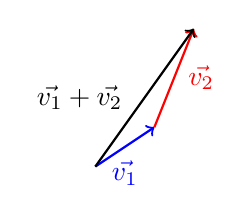
\begin{tikzpicture}[xscale=0.25,yscale=0.25]
        \draw[->,red,thick] (0,-1) -- (2,4) node[midway,right=0.5mm] {$\vec{v_2}$};
        \draw[->,blue,thick] (-3,-3) -- (0,-1) node[midway,below=0.5mm] {$\vec{v_1}$};
        \draw[black,->,thick] (-3,-3) -- (2,4) node[midway,left=1.5mm] {$\vec{v_1}+\vec{v_2}$};
    \end{tikzpicture}
    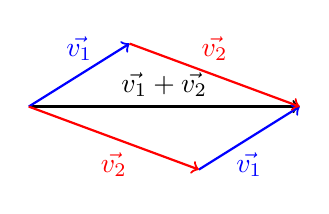
\begin{tikzpicture}[xscale=0.4,yscale=0.4]
        \draw[->,black,thick] (-4.3,0) -- (4.3,0) node[midway,above] {$\vec{v_1}+\vec{v_2}$};
        \draw[->,blue,thick] (-4.3,0) -- (-1.1,2) node[midway,above=0.5mm] {$\vec{v_1}$};
        \draw[->,blue,thick] (1.1,-2) -- (4.3,0) node[midway,below=0.5mm] {$\vec{v_1}$};
        \draw[->,red,thick] (-1.1,2) -- (4.3,0) node[midway,above=0.5mm] {$\vec{v_2}$};
        \draw[->,red,thick] (-4.3,0) -- (1.1,-2) node[midway,below=0.5mm] {$\vec{v_2}$};
    \end{tikzpicture}
\end{figure}
Now, let's understand the concept of a scalar multiple. A scalar multiple is a non-zero scalar being multiplied by a vector. For example, using $\vec{v_1}$ above, multiplying the vector by a scalar would mean multiplying $\vec{v_1}$ by a non-zero real constant $k$ (where $k$ could equal $2$, $\dfrac{1}{5}$, $\sqrt{3}$,$-1$, etc.). Mathematically, given $\vec{v_1}=<a,b>$, we define the scalar multiply by a factor of $k$ as $k\vec{v_1}=<ka,kb>$. Below is a depiction if $k=3$: 

\begin{figure}[!h]
    \centering
    \hspace{\stretch{1}}
    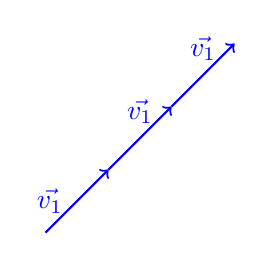
\begin{tikzpicture}[xscale=0.4,yscale=0.4]
        \draw[.->,blue,thick] (-3,-3) -- (-1,-1) node[midway,left=0.5mm] {$\vec{v_1}$};
        \draw[.->,blue,thick] (-1,-1) -- (1,1) node[midway,above=0.5mm] {$\vec{v_1}$};
        \draw[.->,blue,thick] (1,1) -- (3,3) node[midway,above=0.5mm] {$\vec{v_1}$};
    \end{tikzpicture} \hspace{\stretch{1}} $\to$ \hspace{\stretch{1}}
    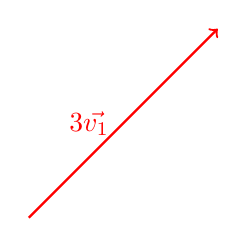
\begin{tikzpicture}[xscale=0.4,yscale=0.4]
        \draw[.->,red,thick] (-3,-3) -- (3,3) node[midway,left=0.5mm] {$3\vec{v_1}$};
    \end{tikzpicture}
    \hspace{\stretch{1}}
\end{figure}

Here is a picture of what would happen if $k<0$.  It would flip the direction of the vector.

\begin{figure}[!h]
    \centering
    \hspace{\stretch{1}}
    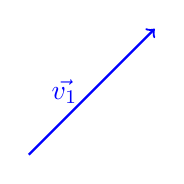
\begin{tikzpicture}[xscale=0.4,yscale=0.4]
        \draw[.->,blue,thick] (-2,-2) -- (2,2) node[midway,left=0.5mm] {$\vec{v_1}$};
    \end{tikzpicture} \hspace{\stretch{1}} $\to$ \hspace{\stretch{1}}
    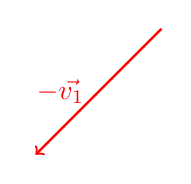
\begin{tikzpicture}[xscale=0.4,yscale=0.4]
        \draw[.->,red,thick] (2,2) -- (-2,-2) node[midway,left=0.5mm] {$-\vec{v_1}$};
    \end{tikzpicture}
    \hspace{\stretch{1}}
\end{figure}

Now, let's learn to subtract the vectors.  Essentially, we need to do the "head-to-tail" method in reverse. Mathematically, given $\vec{v_1}=<a,b>$ and $\vec{v_2}=<c,d>$, we get $$\vec{v_1}-\vec{v_2}=\vec{v_1}+(-\vec{v_2})=<a,b>+<-c,-d>=<a-c,b-d>.$$ Below is the graphical representation.
\begin{figure}[!h]
    \centering
    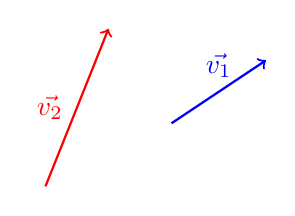
\begin{tikzpicture}[xscale=0.4,yscale=0.4]
        \draw[->,red,thick] (-3,-3) -- (-1,2) node[midway,left=0.5mm] {$\vec{v_2}$};
        \draw[->,blue,thick] (1,-1) -- (4,1) node[midway,above=0.5mm] {$\vec{v_1}$};
    \end{tikzpicture}
    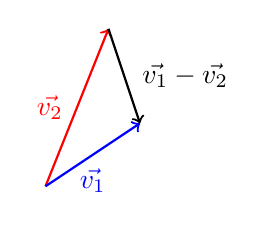
\begin{tikzpicture}[xscale=0.4,yscale=0.4]
        \draw[->,red,thick] (-3,-3) -- (-1,2) node[midway,left=0.5mm] {$\vec{v_2}$};
        \draw[->,blue,thick] (-3,-3) -- (0,-1) node[midway,below=0.5mm] {$\vec{v_1}$};
        \draw[->,black,thick] (-1,2) -- (0,-1) node[midway,right=1mm] {$\vec{v_1}-\vec{v_2}$};
    \end{tikzpicture}
\end{figure}

Now you may be wondering, what if I want to multiply two vectors? Do I just multiply the components of $\vec{v_1}$ and $\vec{v_2}$? Well, the thing is you can, but not in the way you are thinking.  In vector multiplication, there exist two types of answers: \textit{Dot} products and \textit{Cross} products. You can learn more about these on your own, but I am letting you know they exist.

Finally, there is no such thing as vector division. What a letdown. 

The next thing we wish to do with vectors is decompose them into their components.  Sometimes, we're not always given vectors in the nice form $<a,b>$.  Sometimes, we have to extract them out of word problems.

Let's do this one by example.
\begin{example}
Simon kicked a soccer ball at a $15$-degree angle above the horizontal, and the ball is now going at $20$ miles per hour, find the horizontal and vertical components of the ball's velocity.
\end{example}
\begin{solution}
We first draw the diagram indicating the ball's velocity.  This is shown at the top of the next page.

\begin{figure}[!h]
    \centering
    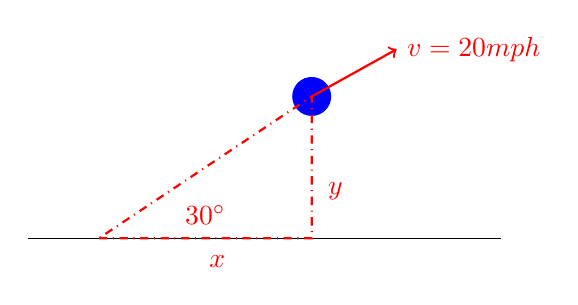
\begin{tikzpicture}[xscale=0.6,yscale=0.6]
        \draw (-5,0) -- (5,0);
        \filldraw[blue] (1,3) circle[radius=0.4];
        \draw[red,->,thick] (1,3) -- (2.8,4) node[right] {$v=20 \text{mph}$};
        \draw[red,dashdotted,thick] (-3.5,0) -- (1,0) -- (1,3) -- (-3.5,0);
        \draw[red] (-1,-0.5) node {$x$};
        \draw[red] (1.5,1) node {$y$};
        \draw[red] (-1.25,0.5) node{$30^{\circ}$};
    \end{tikzpicture}
\end{figure}

\noindent Using trigonometry from \hyperlink{chapter.12}{Chapter 12}, we can find the values of the components: \begin{align*}
    \cos(30^{\circ})&=\dfrac{x}{20} \implies x=20\cos(30^{\circ}) \\
    \sin(30^{\circ})&=\dfrac{y}{20} \implies y=20\sin(30^{\circ})
\end{align*}
Writing this in vector form, we obtain $<20\cos(30^{\circ}),20\sin(30^{\circ})>$. $\Box$
\end{solution}
Now that we know how to decompose a vector into components, what if we need to combine the components? We have a special term for this, called the \textit{magnitude}. The magnitude is denoted as $||\vec{v}||$ and represents the length of a vector (essentially the hypotenuse). This means that we can use the Pythagorean Theorem to find the hypotenuse.  This gives us a new formula for vectors: $$||\vec{v}||=\sqrt{x^2+y^2}.$$
And we can use this magnitude to actually calculate unit vectors for given vectors. For example, by dividing the magnitude of the vector by the vector itself, we obtain the unit vector. This means that the unit vector is $\dfrac{\vec{v}}{||\vec{v}||}=<\dfrac{x}{\sqrt{x^2+y^2}},\dfrac{y}{\sqrt{x^2+y^2}}>$.  To ensure that it's a unit vector, we can take the magnitude and it should be $1$ (it is!).
\section{Modeling Real-World Scenarios}
\noindent This section will explore real-world applications of methods learned in Algebra II and in the previous sections.  Here are some definitions you need to know before we get started: \begin{itemize}
    \item \textit{Displacement}: Change of position of an object relative to the origin.
    \item \textit{Velocity}: Change in position over time.
    \item \textit{Acceleration}: Change in velocity over time.
\end{itemize}
We are going to relate these values in a series of equations called \textit{kinematic equations} to model traveling objects. Here are the five variables we need: $$\begin{matrix} v_i=\text{initial velocity} & v_f=\text{final velocity} & t=\text{time} \\ a=\text{acceleration} & \Delta x=\text{displacement} \end{matrix}$$ Here are the five equations we need to use: $$\begin{matrix} v_f=v_i+at & \Delta x=\left(\dfrac{v_i+v_f}{2}\right)t & \Delta x=v_it+\dfrac{1}{2}at^2 \\ \Delta x=v_ft-\dfrac{1}{2}at^2 & v_f^2=v_i^2+2a\Delta x\end{matrix}$$
Notice that all these equations have one of the five variables missing.  This means that we only three pieces of information to find all five (be sure to see why!).  With these equations, we can basically model any equation provided the acceleration is constant.

Here is a general problem-solving strategy to solve kinematic equations: \begin{enumerate}
    \item Determine an origin for the problem,
    \item Write down known quantities,
    \item Choose the appropriate equation,
    \item Plug in known values,
    \item Solve for the desired variable.
\end{enumerate}
So where are the vectors in this process? The vectors come in all the variables.  Velocity, displacement, and acceleration are all vectors; however, for these equations we are consolidating to one direction of motion.  This means we are only dealing with their components rather than the entire vector.

Let's work out some examples.
\begin{example}
Josh startes from rest and accelerates down a football field at $3.20 \frac{\text{m}}{\text{s}^2}$ for $32.8$ seconds until his foot gives out and he trips.  How fast was he going when he tripped? (Assume Josh runs with constant acceleration.)
\end{example}
\begin{solution}
Let's first draw a picture of the area and an origin for the problem. Typically denote the object in motion as a ball or a block; this case, we use a ball.

\begin{figure}[!h]
    \centering
    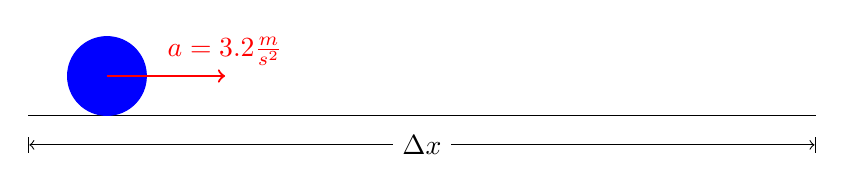
\begin{tikzpicture}[xscale=0.5,yscale=0.5]
        \draw (-10,0) -- (10,0);
        \filldraw[blue] (-8,1) circle[radius=1];
        \draw[->,red,thick] (-8,1) -- (-5,1) node[above] {$a=3.2 \frac{\text{m}}{\text{s}^2}$};
        \draw[|<->|] (-10,-0.75) -- (10,-0.75) node[fill=white,midway] {$\Delta x$};
    \end{tikzpicture}
\end{figure}

For this problem, let's say that Josh is running away from the origin.  We now write down the known quantities: $$a=3.2 \hspace{15mm} t=32.8 \hspace{15mm} v_i=0\text{ (rest)} \hspace{15mm} v_f=\text{?} \hspace{15mm} \Delta x=\text{?}.$$ 
We see here that we don't have displacement nor final velocity.  To solve for final velocity using the variables we have, we choose the $v_f=v_i+at$ equation since it has the known variables, doesn't include the variable we don't have, and includes the variable we want. Substituting values, we get $$v_f=0+(32.8)(3.2) \implies v_f=104.96\frac{\text{m}}{\text{s}^2}.$$ $\Box$
\end{solution}
So where are the vectors?  Remember that this all occurs in the $\hat{i}$ direction, so we don't need the vectors here since it's all in one direction. To see the equation we used in vector form, we change the vectors to indicate their directions: $$\vec{v_f}=\vec{v_i}+\vec{a}t \implies v_f(\hat{i})=v_i(\hat{i})+a(\hat{i})t.$$ Why doesn't time get a vector component? Time has no direction, meaning it's a scalar not a vector. Time isn't dependent on the origin (or any location) $-$ it passes regardless of where the origin is.

\begin{remark}
Note that the way that $\hat{i}$ is written here is slightly different than how most teachers will write it.  Most teachers, and some other texts, will not write the "dot" above the $i$ and will replace it with the hat.  That is the preferred method of writing it, but certain limitations within the processing software didn't let us do it.
\end{remark}

\begin{note}
The way in which we denoted acceleration can prove to be very confusing later.  In Physics 1, you will be tasked with creating a \textbf{free-body diagram}, which indicates the forces exerted on an object.  Acceleration and are NOT forces, so refrain from using arrows to indicate these on a free-body diagram.   
\end{note}
Let's do another one.  It won't be much harder than the first.
\begin{example}
Cole is an expert car driver. One day, Cole gets into his 2013 Ford Fusion and accelerates at a uniform rate from rest over a time of $5.21$ seconds for a distance of $110$ metres.  He then swiftly merges onto the highway and continues on with his drive.  Determine the acceleration of Cole's 2013 Ford Fusion.
\end{example}
\begin{solution}
Since the diagram for this problem is essentially the same as the previous example, we won't draw a new graph.  Here's the quantities we know: $$v_i=0 \hspace{15mm} t=5.21 \hspace{15mm} \Delta x=110 \hspace{15mm} v_f=\text{?} \hspace{15mm} a=\text{?}.$$
We pick the equation $\Delta x=v_it+\dfrac{1}{2}at^2$ because it doesn't include $v_f$, the one variable we don't care for.  Plugging in numbers and solving for $a$ gives us $$110=0+\dfrac{1}{2}(a)(5.21)^2 \implies a=8.105\frac{\text{m}}{\text{s}^2}.$$ $\Box$
\end{solution}
Again, you could do the vector form for that problem, but it's unnecessary.

We spent the last two problems discussing objects traveling horizontally, but what if an object was travelling vertically (falling)? We could do that too!
\begin{example}
Quinn decides to skydive for his 19$^\text{th}$ birthday. He drops from an altitude of $5000$ metres.  Find Quinn's final velocity as he parachutes safely and find how long he falls for.
\end{example}
\begin{solution}
First, we will find the final velocity.  The setup is the same for both parts.

We first note that to \textit{drop} an object implies that it starts with an initial velocity of zero.  Also, a falling object has the acceleration of the speed of gravity, which is $9.8\frac{\text{m}}{\text{s}^2}$ downward.

Finding the origin is really important since it provides us with the direction of motion.  This ensures that our signs are correct.  Typically, we allow the upward direction to be positive, similar to a coordinate plane.  We can summarize the values we know below: $$a=-9.8 \hspace{15mm} v_i=0 \hspace{15mm} \Delta y=0-5000=-5000 \hspace{15mm} v_f=\text{?} \hspace{15mm} t=\text{?}.$$ To find final velocity, we use the equation $v_f^2=v_i^2+2a\Delta x$.  Plugging the values and solving for $v_f$, we get $$v_f^2=0+2(-9.8)(-5000)=98000 \implies v_f=-313.05\frac{\text{m}}{\text{s}}.$$ Notice how we used a negative value for $v_f$; the velocity vector is also downward (in the direction of motion), which is the negative direction.

Now, we need to find time.  To minimize error, we are going to use the values we were given rather than the one we found; in case we found $v_f$ incorrectly, that means that we won't find $t$ correctly. So, we use the equation $\Delta x=v_it+\dfrac{1}{2}at^2$ to find $t$.  Substituting values, we get $$5000=0+\dfrac{1}{2}(-9.8)(t^2) \implies t=31.94\text{s}.$$ $\Box$
\end{solution}
So what if the problem was in two directions? Could we use the same logic? We can, but now we have to implement the vectors. This will help us ensure that we only cover one direction at a time and do not confuse them.  Since this is beyond the scope of the book, we won't work out an example.  You can find one in the challenge problems if you wish to try one.

Now, let's discuss how to interpret graphs in physics.  It's very similar, but there's some key things to watch out for.
\section{Properties of Graphs}
\noindent This section will cover graphs of functions in physics and how to interpret them.  Most of these graphs will be based on the problems solved along the way, meaning that the graphs will mostly fall into one of three types: \textit{displacement vs. time}, \textit{velocity vs. time}, or \textit{acceleration vs. time}.  We will start with displacement.

Note that these subsections will be summaries of the key details to note rather than completely describing it.  More information will be described in the Physics 1 curriculum.
\textbf{Displacement Versus Time}.  Displacement versus time gives us a plot of the position of the object in two dimensions.  If the object moves further away, the $|y|$ will increase.  If the object moves closer to the origin (starting point), $|y|$ will decrease.

\begin{remark}
Note how we use $|y|$ instead of $y$.  This is because the object could travel in the negative direction, which is possible in motion.  Think about it this way: start at the centre of a football field.  Moving toward the opposing goal is the positive direction, moving toward your goal is the negative direction.
\end{remark}

The slope of this graph represents velocity.  We know this since velocity, by definition, is the change in displacement over time.  If the graph is horizontal, this means that the object is not moving ($v=0$).

If the graph is concave up, there exists a positive acceleration.  When the graph is concave down, there is a negative acceleration.  What is concavity?  Concavity is the slope of the slope, which we can tell by the direction of the curve.  If the curve makes a bowl shape (or a smiley face), we denote this as \textit{concave up}.  If the curve makes an inverted bowl shape (or a frowny face), we denote this as \textit{concave down}.  Below is a picture of both concavities:
\begin{figure}[!h]
    \centering
    \begin{tikzpicture}
        \draw[domain=-6.28:0,scale=1,blue,variable=\x] plot ({\x},{sin(\x/2 r)}) node[midway,below left=0mm and 20mm] {Concave down};
        \draw[domain=0:6.28,scale=1,red,variable=\x] plot ({\x},{sin(\x/2 r)}) node[midway,above right=0mm and 20mm] {Concave up};
        \filldraw (0,0) circle[radius=1pt];
    \end{tikzpicture}
\end{figure}

To find the graph of distance versus time, we can take the absolute value of the graph.
\textbf{Velocity Versus Time}.  Velocity versus time will graph the motion of the object over time.  The slope of this graph gives us acceleration.  When the graph is horizontal, there is no acceleration.  This means the object is moving at constant velocity.  When we take the absolute value of the graph, we obtain the speed versus time graph.

\begin{remark}
Note how are making a stark difference between speed and velocity.  They are not the same!  Velocity is a vector while speed is a scalar.
\end{remark}

\textbf{Acceleration Versus Time}.  This graph models the acceleration versus time of an object.  In most cases, this graph will be flat or piece-wise flat, meaning there is constant acceleration.  In later years of Physics, this graph can change to be any polynomial function over time.  If we find the area under the graph, we find the change in velocity over the interval of time.

Since there wasn't much math going on here, we are only going to do one example.  This will be the peak difficulty for this topic.
\begin{example}
Take the function $a(t)=\begin{cases} 2t & t<4 \\ 1 & t\geq 4 \end{cases}$, where $a(t)$ represents the acceleration function of an object traveling through space.  Assume the particle starts at rest and is positioned at the origin.  Find the corresponding velocity function.
\end{example}
\begin{solution}
For the time $t<4$, we have an increasing acceleration.  This means that over time, the velocity graph is steepening.  What graph do we know that does that? A parabola!  This means that until $t=4$, we have a parabola.  We will match the exact parabola once we discuss the other half.

When $t\geq 4$, we have constant acceleration.  This means that the velocity is steadily increasing over time, just like a line!  This must mean that the velocity is linear.  Now, let's match the two graphs.

At $t=0$, the graph is at rest and starts at the origin.  This means that the vertex of our parabola must be at $(0,0)$.  So, our graph must be $y=t^2$.  For the second half, we know that the constant acceleration of $y=1$ must correlate to exactly $y=t$.

This means that the velocity function, $v(t)=\begin{cases} t^2 & t<4 \\ t & t\geq 4\end{cases}$. $\Box$
\end{solution}
With this, we conclude our discussion of kinematics and physics.  For the next section, we need to learn how to use a graphing calculator $-$ an essential tool in both Pre-calculus and physics.
\section{Using a Graphing Calculator}
\noindent If you haven't bought a graphing calculator yet, you will need one for your time at Suncoast.  We, the authors of this book, recommend a TI-84 Plus Color calculator for high school; for college, we recommend switching to a TI-Nspire CX calculator.  We believe that the TI-Nspire isn't as user-friendly and is too powerful for your needs.  All explanations here will follow a TI-84 Plus Color Calculator.

It is highly unlikely that in the real world, we won't be doing every calculation by hand.  There is too much room for error when a computer can do it faster and with ensured accuracy.

What can we do with this calculator?  We can do a number of things, but we will go through some of the essential topics for physics and pre-calculus.
\subsection{Linear Regression}
\noindent Linear Regression is the process of fitting a line to a given set of data and determining how well that line fits the data.  This is an essential tool for the physics laboratory, because it helps us find fundamental constants given certain equations.

Using a TI-84 Plus Color calculator, follow the steps below to find a linear regression model. \begin{enumerate}
    \item Press the \texttt{MODE} button.  Scroll down until you find \texttt{Stat Diagnostics} and \texttt{Stat Wizards}.  Turn both of these on.  This should be a one-time issue; however, every time your calculator runs out of battery/charge, or is reset, you will need to do this again.
    \item Press the \texttt{STAT} button, then press \texttt{1:Edit}. This should bring up a list of tables titled \texttt{L1}, \texttt{L2}, \texttt{L3}, and so on.  These are the lists your calculator can store.
    \item In list \texttt{L1}, type in all independent variables.  Go to the first empty column of the table, type in a value, then press \texttt{ENTER}.  This will move the cursor to the next row, when you can type in a new value.
    \item Then, press the Right arrow key to move to the next list (\texttt{L2}).  Type in all the dependent variables that correspond with each independent variable.
    \item Press \texttt{2ND}, then \texttt{MODE}.  This is the Quit button, and will return you to the home screen.
    \item Press the \texttt{STAT} button again. Press the Right arrow to move to the \texttt{CALC} window.  Click on \texttt{8:LinReg(a+bx)}.
    \item On this window, there are a few options.  \texttt{XList} represents the independent variable list (which is correctly \texttt{L1} by default), \texttt{YList} represents the dependent variable list (\texttt{L2} by default), \texttt{FreqList} which is unimportant to us, \texttt{Store ReqEq} which is important, then finally the \texttt{Calculate} button.
    \item Move your cursor to \texttt{Store RegEq}.  Press the \texttt{ALPHA} buttom, then press \texttt{TRACE}.  This will bring up a drop-down menu containing equation names (\texttt{Y1}, \texttt{Y2}, \texttt{Y3}, and so on).  Press \texttt{1:Y1}.  Now, press \texttt{Calculate}.
    \item The next window will tell you all the important statistics.  \texttt{a=} will be the $y$-intercept and \texttt{b=} will be the slope.  A constant called \texttt{r} will also be there; this represents how well the line fit the data.  The closer it is to $-1$ or $1$, the more linear the data was.  If it's close to $0$, the data is not linear.
    \item To see a visual of the data, press \texttt{2ND} then \texttt{Y=}.  Press \texttt{Plot 1}, ensure that the \texttt{XList} and \texttt{YList} are correct, then press the Scatterplot graph.  Then, press \texttt{ZOOM}, then \texttt{9:ZoomStat}.  This will bring up a graph of the scatter-plot and the regression line.
    \item Press \texttt{2ND}, then \texttt{MODE} to return to the home screen.
\end{enumerate}

\begin{remark}
To delete a list, you can go to the lists menu, scrolling up to a list, then pressing \texttt{CLEAR}, then \texttt{ENTER}.  DO NOT press \texttt{DELETE}.  This will delete the list.  To delete an entry, press \texttt{DELETE} on the entry.
\end{remark}

Now that we've explained this, we can look at some problems.
\begin{example}
Below is a set of data representing the resistance provided a resistor in a circuit depending n the length ($l$) and cross-sectional area ($A$).  Determine the value of the constant $\rho$ using the equation $R=\rho\dfrac{l}{A}$.
\begin{table}[!h]
    \centering
    \begin{tabular}{|c||c|c|c|c|}
        \toprule
        Cylinder & $A$ ($m^2$) & $l$ ($m$) & $\Delta V$ ($V$) & $R$ ($\Omega$) \\
        \midrule
        $1$ & $0.00049$ & $0.030$ & $1.02$ & $23.6$ \\
        $2$ & $0.00049$ & $0.050$ & $2.34$ & $31.5$ \\
        $3$ & $0.00053$ & $0.080$ & $3.58$ & $61.2$ \\
        $4$ & $0.00057$ & $0.150$ & $6.21$ & $105$ \\
        \bottomrule
    \end{tabular}
\end{table}
\end{example}
\begin{solution}
The equation given doesn't represent a line very well.  There's a fraction!  Well, what we can do is create a new line of data (via a substitution) that will make this linear.  If we set $\dfrac{l}{A}$ to be the independent variable, we can find $\rho$ by finding the slope of the resulting line.  Let's extend the table to find this value.
\begin{table}[!h]
    \centering
    \begin{tabular}{|c||c|c|c|c||c|}
        \toprule
        Cylinder & $A$ ($m^2$) & $l$ ($m$) & $\Delta V$ ($V$) & $R$ ($\Omega$) & $\frac{l}{A}$ ($m^{-1}$)\\
        \midrule
        $1$ & $0.00049$ & $0.030$ & $1.02$ & $23.6$ & $0.030/0.00049$ \\
        $2$ & $0.00049$ & $0.050$ & $2.34$ & $31.5$ & $0.050/0.00049$ \\
        $3$ & $0.00053$ & $0.080$ & $3.58$ & $61.2$ & $0.080/0.00053$ \\
        $4$ & $0.00057$ & $0.150$ & $6.21$ & $105$ & $0.150/0.00057$ \\
        \bottomrule
    \end{tabular}
\end{table}

\begin{remark}
The reason we didn't do the calculations is because the calculator can do them within the table, so it saves us time to leave it like this.
\end{remark}

Using the data for $\dfrac{l}{A}$ as the independent variable, along with the values of $R$ as the dependent variable.  Performing the steps shown above, we can find the equation of the line of be $$y(x)=-5.204+0.419(x).$$ So many people might be asking how there's a $y$-intercept if the equation was supposed to be in the form $y=kx$.  In real-life, there's always outside factors that offset the values, which impact the accuracy of the data.  We can't have negative resistivity ($\rho$), so this is a part of the domain we ignore.

What we can analyze is that the resistivity is about $0.419$. $\Box$
\end{solution}
Let's keep the ball rolling and do another example.
\begin{example}
Consider the data below relating the voltage of a battery to the current yielded and the resistance within the circuit.  Using the equation $\Delta V=IR$, determine the value of the resistance.
\begin{table}[!h]
    \centering
    \begin{tabular}{|c||c|c|c|c|c|c|}
    \toprule
        $\Delta V$ ($V$) & $6.0$ & $5.0$ & $3.5$ & $2.5$ & $2.0$ & $1.5$ \\
        $I$ ($A$) & $0.078$ & $0.070$ & $0.044$ & $0.036$ & $0.027$ & $0.018$ \\
        \bottomrule
    \end{tabular}
\end{table}
\end{example}
\begin{solution}
Fortunately, for this example, we don't need to do any manipulation since the function is already linear.  When we do linear regression, we know that the independent variable will be current ($I$) and the dependent variable will be voltage ($\Delta V$).

When we follow the process above, we get the following equation: $$y(x)=3.008+12.086(x).$$ This means that the resistance of the circuit is $12.086\Omega$. $\Box$
\end{solution}
One last example; trust me, this one will be much harder.
\begin{example}
The table below gives values of $\theta_i$ and $\theta_r$, angles of reflection of light between two mediums.  Using the table and the equation $\sin(\theta_i)=n_r\sin(\theta_r)$, determine the constant $n_r$.

\begin{table}[!h]
    \centering
    \begin{tabular}{|c||c|c|c|c|c|}
        \toprule
        Trial & $1$ & $2$ & $3$ & $4$ & $5$ \\
        \midrule
        $\theta_i$ & $30^{\circ}$ & $40^{\circ}$ & $50^{\circ}$ & $60^{\circ}$ & $70^{\circ}$ \\
        $\theta_r$ & $20^{\circ}$ & $27^{\circ}$ & $32^{\circ}$ & $37^{\circ}$ & $40^{\circ}$ \\
        \bottomrule
    \end{tabular}

\end{table}
\end{example}
\begin{solution}
This equation is almost linear, but we need to make some small adjustments.  We know that we need to find $n_r$, which will be the slope of the graph.  This means that $\sin(\theta_r)$ will be the independent variable and $\sin(\theta_i)$ will be the dependent variable.  So, we need to extend the table to input these values.

\begin{table}[!h]
    \centering
    \begin{tabular}{|c||c|c|c|c|c|}
        \toprule
        Trial & $1$ & $2$ & $3$ & $4$ & $5$ \\
        \midrule
        $\theta_i$ & $30^{\circ}$ & $40^{\circ}$ & $50^{\circ}$ & $60^{\circ}$ & $70^{\circ}$ \\
        $\theta_r$ & $20^{\circ}$ & $27^{\circ}$ & $32^{\circ}$ & $37^{\circ}$ & $40^{\circ}$ \\
        $\sin(\theta_i)$ & $\sin(30^{\circ})$ & $\sin(40^{\circ})$ & $\sin(50^{\circ})$ & $\sin(60^{\circ})$ & $\sin(70^{\circ})$ \\
        $\sin(\theta_r)$ & $\sin(20^{\circ})$ & $\sin(27^{\circ})$ & $\sin(32^{\circ})$ & $\sin(37^{\circ})$ & $\sin(40^{\circ})$ \\
        \bottomrule
    \end{tabular}

\end{table}
Following the steps for linear regression, we find that the function we need is $$y(x)=-0.008+1.460(x).$$  This means that the value of the constant is about $1.460$. $\Box$
\end{solution}
This is all we need to cover for this topic.  Now, for the next thing that the graphing calculator can do: calculate roots of a polynomial and solve systems of linear equations.
\subsection{Polynomial Root Finder \& Simultaneous Equation Solver}
\noindent By default on a TI-84 Plus Color, there is an app called \texttt{PolySmlt 2} that can do both functions named in the subsection title.  This is extremely useful for speeding up problems that involve these steps (trust me, they're everywhere in physics).

\begin{remark}
Note that these apps will disappear if you clear your Archive memory from your calculator.  DO NOT do that! It's a hassle to reinstall.
\end{remark}

So how do we use these?  Here are the steps for the Polynomial Root finder:\begin{enumerate}
    \item Press the \texttt{APPS} button.  This should bring a menu with a list of default apps on your calculator.
    \item Locate the \texttt{PolySmlt 2} app.  It could be anywhere on the list, usually it's somewhere around Number 8.
    \item Opening the app opens a start menu, which you can press \texttt{ENTER} to get through, and then a menu listing the two options.  Press \texttt{1:Polynomial Root Finder}.
    \item In this next menu, you can list the properties of the polynomial.  The main property on this menu is the degree (order) of the polynomial. Be sure to put the right degree.  Also, scroll down and press \texttt{a+bi} in the second row.  We want the root finder to list any complex roots that it may find.
    \item Press \texttt{GRAPH} to move to the next window.  This window allows you to type in the coefficients of the polynomial from highest to lowest degree.  Be sure to include any $0$'s if any.
    \item Press \texttt{GRAPH} to find the roots.  The resulting window has the roots of the polynomial.
    \item When you are finished, press \texttt{Y=} to return to the main menu.
\end{enumerate}
Here are the steps for the Simultaneous Equation solver: \begin{enumerate}
    \item On the main menu of the app, press \texttt{2:SimultEqn} to open this function.
    \item In this window, press the number of equations you have and the number of unknowns you need to find.  For this to work, the number of equations must be at least the number of unknowns.  You'll learn more about what happens if not when you take Linear Algebra.
    \item Press \texttt{GRAPH} to move to the next window.  This window brings up a large matrix with all entries as $0$.  We fill this in using the coefficients of the system, where the column after the darker line is the constant at the end.  (For example, if the system was $\begin{cases} x+y=2 \\ x-2y=7\end{cases}$, the first row would be $1$ | $1$ | $2$ and the second row would be $1$ | $-2$ | $7$).
    \item Press \texttt{GRAPH} to solve the system. The resulting window has the solution to the system.
    \item When you are finished, press \texttt{Y=} to return to the main menu.
\end{enumerate}
You can play around with these all you want; you can use these to check your answers from problems throughout the book if you want.

With this, we conclude our discussion of calculator tricks and our study of physics.  If you want to learn more about how to use it, its more advanced functionality (such as programming), the Internet has loads of resources.  Also, you can feel free to reach out to Mr. Ellis using the email in the introduction about programming.
\begin{reviewset}
\item An engineer is designing the runway for an airport. Of the planes that will use the airport, the lowest acceleration rate is likely to be $3\frac{\text{m}}{\text{s}^2}$. The takeoff speed for this plane will be $65\frac{\text{m}}{\text{s}}$. Assuming this minimum acceleration, what is the minimum allowed length for the runway? 
\item A bullet leaves a rifle with a muzzle velocity of $521\frac{\text{m}}{\text{s}}$. While accelerating through the barrel of the rifle, the bullet moves a distance of $0.840 m$. Determine the acceleration of the bullet (assume a uniform acceleration).
\item Below is an experiment to determine the value of a constant $nR$ given Pressure ($P$), Volume ($V$), and Temperature ($T$) of an ideal gas.  Using the table and the equation $PV=nRT$, determine the value of this constant.
\begin{table}[!h]
    \centering
    \begin{tabular}{|c||c|c|c|c|c|c|c|}
    \toprule
    Trial & $1$ & $2$ & $3$ & $4$ & $5$ & $6$ & $7$ \\
    \midrule
        $V$ ($cm^3$) & $4.0$ & $3.0$ & $5.0$ & $4.0$ & $10.0$ & $5.0$ & $3.0$ \\
        $P$ ($kPa$) & $250$ & $330$ & $220$ & $270$ & $110$ & $230$ & $380$\\
        $T$ ($^{\circ}C$) & $0$ & $0$ & $20$ & $20$ & $20$ & $40$ & $40$ \\
    \bottomrule
    \end{tabular}
\end{table}
\end{reviewset}
\begin{challengeset}
\item Suppose Matthew kicks a ball at $45^\circ$ with respect to the horizontal with a speed of $30$ metres per second. Find how long it takes the ball to fall down, and how far the ball goes.
\item Suppose we have two trains and a bee. One train starts at a distance $d$ away from the other train. Both trains travel at constant speed $v$, but in opposite directions towards each other. Suppose there is a bee that travels at a constant speed $c$ where $c>v$. So this bee starts off at one train and flies to the other train. Upon reaching the other train, the bee switches direction and maintains the same velocity $c$ until it reaches the original train, and switches direction once more. This cycle repeats until the trains crash. What is the total distance the bee travels by the time the trains crash?
\item Below is a table of data found in an experiment that shoots a ball of mass $m$ to a height $h$ using a spring that compresses $k$ metres.  Using the table below, and the equation $h=\dfrac{kx^2}{mg}$, determine the value of the spring constant $k$. (Note that the ball has a uniform compression distance of $x=0.020$ and gravity is also constant.)

\begin{table}[!h]
    \centering
    \begin{tabular}{|c||c|c|c|c|c|}
        \toprule
       $m$ ($kg$) & $0.020$ & $0.030$ & $0.040$ & $0.050$ & $0.060$ \\
       $h$ ($m$) & $0.49$ & $0.34$ & $0.28$ & $0.19$ & $0.18$ \\
       \bottomrule
    \end{tabular}
\end{table}
\end{challengeset}
\end{document}
